\documentclass[apj]{emulateapj}

\usepackage{biblatex}
\addbibresource{biblio.bib}

\usepackage{graphicx}
\usepackage{epsfig}
\usepackage{amssymb,amsmath}
\usepackage{array}
\usepackage{threeparttable}


\singlespace

%definitions
\newcommand{\Msol}{${\rm M_{\sun}}$}


%% Editing markup...
\usepackage{color}


%%%%%%%%%%%%%%%%%%%%%%%%%%%%%%%%%%%%%%%%%%%%%%%%%%%%%%%%%%%%%%%%%%%%%%%%%%%
% WARNING: This LaTeX block was generated automatically by authors.py
% Do not change by hand: your changes will be lost.

%%%%%%%%%%%%%%%%%%%%%%%%%%%%%%%%%%%%%%%%%%%%%%%%%%%%%%%%%%%%%%%%%%%%%%%%%%%


% --------------------- Ancillary information ---------------------
\shortauthors{Horlaville, P.}
\shorttitle{Horlaville+2022}
\slugcomment{Draft: \today}


\begin{document}

\title{Exploring Line Intensity Cube Predictions with \MakeLowercase{\texttt{limlam$\_$mocker}}}
%Investigating Dark Matter Halos Through Line Intensity Fluctuations
 %% ---------
 
\author{Patrick Horlaville\altaffilmark{1}}
\altaffiltext{1}{CITA, University of Toronto}
 
\keywords{cosmology: galaxy --- dark matter --- CO line intensity}



\section{Introduction}
\label{sec:intro}
\subsection{Background}
The study of high redshift galaxies is increasingly important in the context of our understanding of galaxy formation and cosmology. While modern surveys still struggle to efficiently probe those populations, simulation techniques such as intensity mapping have proven to be able to infer the properties of those dear high redshift galaxies, \textit{e.g}. intensity mapping of carbon monoxide and its ground-state CO(1-0) transition (Li et al., 2016) \cite{Li_2016}.

Intensity mapping (IM), or line intensity mapping (LIM), is a technique that consists of probing the 3D sky (RA, DEC \& $z$) at low angular resolution of specific molecular lines \cite{Karkare}. The strength of this analysis resides in 1) its potential to probe large cosmological volume quickly and 2) its ability to probe galaxies invisible to standard galaxy surveys. 

\subsection{Related to the Project}

The goal of this project is to analyze how predicted galaxies' properties as found by Li et al. (2016) \cite{Li_2016} compare to those of a Python program named \texttt{limlam$\_$mocker}. The two aim to perform a line intensity analysis using CO emission over dark matter halos, which allows to compute their CO brightness temperature. However, two main differences are to be considered. First, the average redshift of the probed halos are not the same. Second, the method used to identify those halos are not the same. This will be elaborated upon later.

Both analyses consider a minimum cutoff for halos' mass since low-mass halos are not expected to be CO-bright as they are expected to be poor of systems rich in dust or metal (Li et al., 2016) \cite{Li_2016}. We can hence look into how does the CO brightness temperature depend on the chosen mass cutoff. The final objective of this project would be to use \texttt{limlam$\_$mocker} to determine this relationship and compare it to the result of Li et al. (2016). 


\section{Process}
\label{sec:data}
Explaining the \texttt{limlam$\_$mocker} program


\subsection{Subsection 1}
\label{sec:cmb_data}
This is a sub-section.
Here is an equation:
\begin{equation}
E = mc^2
\label{eq:relativity}
\end{equation}
Here is an example of math-mode in the main text: $a^2 + b^2 = c^2$.  Here is a reference, to Fig.~\ref{fig:figureOfSpectrum}.  The data section is section \ref{sec:data}.


\begin{figure}[!h]
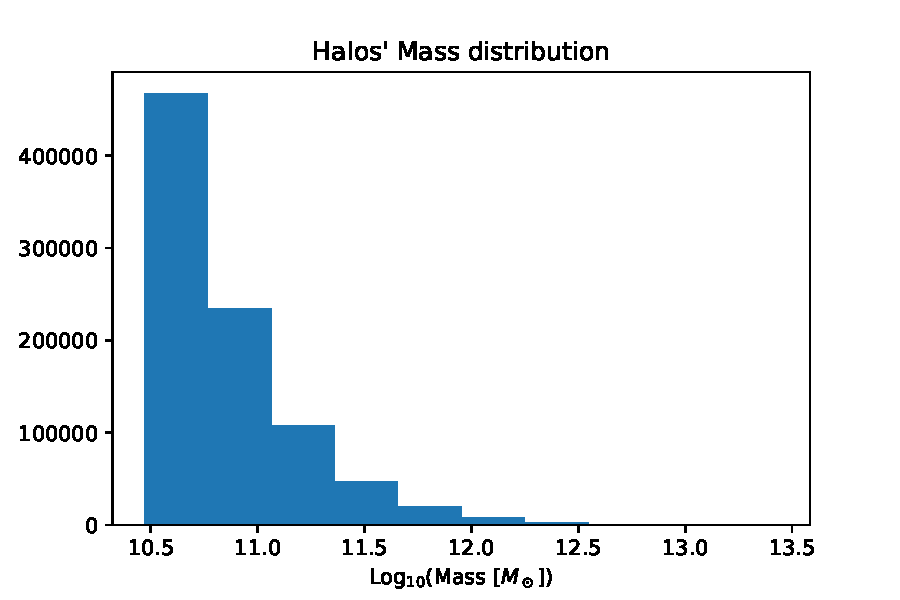
\includegraphics[width=1.05\columnwidth]{mass_distribution.pdf}
\caption{Here shown is the distribution of halos' masses from the catalog used in our \texttt{limlam}\_\texttt{mocker} analysis.\vspace{1mm}}
\label{fig:figureOfSpectrum}
\end{figure}



\begin{table}[!h]
\begin{center}
\begin{threeparttable}
\caption{A table.}
\begin{tabular}{|l|c|c|}
\hline 
Col 1 & Col 2 & Col 3 \\
 \hline  
Val 1 & Val 2 & Val 3 \\
Val 1 & Val 2 & Val 3 \\
\hline
\end{tabular} 
\vskip 2mm
\begin{tablenotes} \item  
\begin{center}
\begin{flushleft}
Description of table.
\end{flushleft}
\end{center}
\end{tablenotes}
\label{tab:vitalStats_kappa}
\end{threeparttable}
\end{center}
\end{table}


\printbibliography

%\acknowledgments

%% %% \bibliographystyle{act}
%% \bibliographystyle{apj}

%% \bibliography{lenscib_refs.bib,apj-jour}



\end{document}
